\section{Results}\label{sec:results}

All numbers are on outer test units. Calibration sets had 32 units (FD001, FD003, N-CMAPSS), 39 (battery), 70 (PHM08), 80 (FD004) and 83 (FD002) under cross-validation. Unless stated, rates are averaged over the three repetitions of the proper-training/calibration split, and tests use repetition~0, in which every unit is tested once.

\subsection{The guarantee holds; interval calibration does not deliver it}\label{sec:res-valid}

Table~\ref{tab:validity} and Fig.~\ref{fig:validity} give the failure-before-replacement rate at the primary lead time. With $\alpha=0.10$ the conformal notice alarm failed on 6.0--11.7\,\% of test units across the seven datasets, and with $\alpha=0.05$ and $0.20$ on 1.3--5.1\,\% and 14.3--20.6\,\%. Pooled over the seven datasets, four lead times and three repetitions (13,788 unit--cell evaluations), the rates were 3.8, 9.3 and 19.4\,\% for nominal 5, 10 and 20\,\%. In repetition~0 no exact binomial test of rate $>0.10$ was significant after Holm's correction (smallest adjusted $p=0.84$), so H1 is supported on all seven datasets. Rates slightly above 10\,\% (FD003 11.7\,\%, N-CMAPSS 11.1\,\%, battery 10.6\,\%, FD004 10.4\,\%) are within sampling error; for distinct critical levels the expected rate is $(n+1-q)/(n+1)$, 9.1\,\% with 32 calibration units and 10.0\,\% with 39.

The interval-calibrated alarm on the same signal and trigger did not deliver its nominal level. Calibrated with residuals over all rows (LB-all), the lower-bound alarm at nominal 10\,\% failed on 18.2\,\% (N-CMAPSS) to 69.6\,\% (battery) of units, 46.6\,\% pooled, with $p<0.005$ on every dataset (H2 supported, 7 of 7). Rows far from failure, where the capped target makes residuals small, dominate the pooled residual quantile, so the bound is tight far from failure and loose at the stopping time. Restricting the residuals to rows with $r_t\le c$ (LB-near) brought the rate close to nominal on six datasets (4.0--8.6\,\%) but not on N-CMAPSS (15.2\,\%, and 17.8\,\% at the longest lead time), and its level depends on how the evaluator chooses the rows. The guarantee costs notice: at $\alpha=0.10$ CNA alarms left a median of 15--17 engine cycles at a lead time of 10, against 11--12 for LB-all; on the battery cells 43 cycles at a lead time of 30.

Corollary~\ref{cor:pac} predicts more than the mean. Across the 105 calibration sets at the primary lead time (seven datasets, five folds, three repetitions), the number of failures among the test units of a fold followed the Beta-binomial law that the corollary implies: the randomised probability integral transforms were consistent with uniformity (Kolmogorov--Smirnov $p=0.93$ at $\alpha=0.10$; 0.53 and 0.70 at 0.05 and 0.20), the variance of the fold-level failure rate at $\alpha=0.10$ was 0.0049 against 0.0048 predicted, and 103 of the 105 rates lay inside the 90\,\% predictive band (Fig.~\ref{fig:conditional}). For folds of 20--25 units the band reaches 25--26\,\%: a valid 10\,\% alarm can show more than twice its nominal rate on a test of that size. This check was not in the protocols, and folds of one repetition share calibration units, so the $p$-values are descriptive.

\begin{table*}[t]\footnotesize\setlength{\tabcolsep}{4.5pt}
\caption{Failure before the planned replacement at the primary lead time (10 cycles; battery 30 cycles), five-fold cross-validation, mean of three repetitions. Second column: repetition~0 for CNA at $\alpha=0.10$ (failures; rate; Clopper--Pearson 95\,\% interval). Last column: median notice at the alarm (cycles), CNA 0.10 / LB-all 0.10.}\label{tab:validity}
\resizebox{\textwidth}{!}{%
\begin{tabular}{@{}lllllllll@{}}
\toprule
Dataset (test units) & CNA 0.10, rep.~0 & CNA 0.05 & CNA 0.10 & CNA 0.20 & CNA-DA & LB-all 0.10 & LB-near 0.10 & Notice \\
\midrule
PHM08 (218) & 18 (0.083; 0.050--0.127) & 0.034 & 0.086 & 0.177 & 0.009 & 0.446 & 0.080 & 16 / 11 \\
FD001 (100) & 7 (0.070; 0.029--0.139) & 0.013 & 0.060 & 0.143 & 0.013 & 0.333 & 0.043 & 17 / 12 \\
FD002 (260) & 20 (0.077; 0.048--0.116) & 0.042 & 0.088 & 0.191 & 0.008 & 0.381 & 0.040 & 15 / 12 \\
FD003 (100) & 14 (0.140; 0.079--0.224) & 0.027 & 0.117 & 0.197 & 0.027 & 0.480 & 0.063 & 16 / 11 \\
FD004 (249) & 31 (0.124; 0.086--0.172) & 0.051 & 0.104 & 0.206 & 0.011 & 0.466 & 0.086 & 16 / 11 \\
N-CMAPSS (99) & 11 (0.111; 0.057--0.190) & 0.037 & 0.111 & 0.178 & 0.057 & 0.182 & 0.152 & 23 / 19 \\
Battery (123) & 15 (0.122; 0.070--0.193) & 0.033 & 0.106 & 0.198 & 0.011 & 0.696 & 0.070 & 43 / 28 \\
\bottomrule
\end{tabular}}
\end{table*}

\begin{figure*}[t]\centering
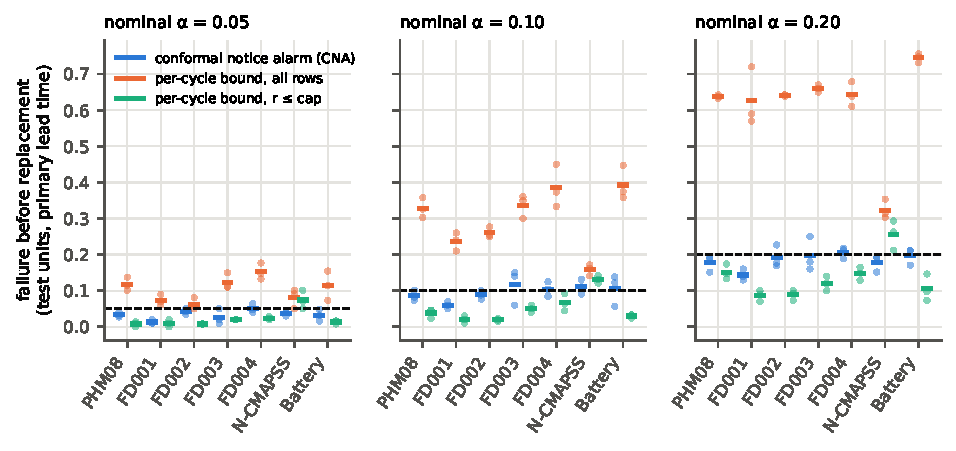
\includegraphics[width=0.95\textwidth]{figures/Fig2_validity.pdf}
\caption{Failure before the planned replacement at the primary lead time (10 cycles; battery 30) for the conformal notice alarm (CNA) and per-cycle split-conformal lower-bound alarms on the same signal and trigger, at three nominal levels (dashed). Dots: the three repetitions; bars: their mean. Five-fold cross-validation.}\label{fig:validity}
\end{figure*}

\begin{figure}[t]\centering
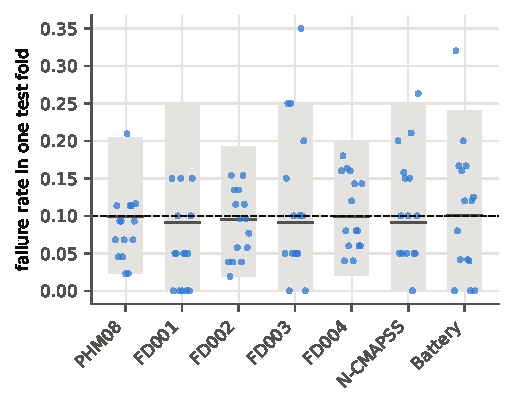
\includegraphics[width=\linewidth]{figures/Fig3_conditional.pdf}
\caption{Failure rate of CNA ($\alpha=0.10$, primary lead time) in each of the 105 test folds (five folds, three repetitions per dataset) against the Beta-binomial law of Corollary~\ref{cor:pac}: 90\,\% predictive band for the median fold size (grey) and its mean $(n+1-q)/(n+1)$ (line).}\label{fig:conditional}
\end{figure}
